\chapter{Introduction}
\section{The Spherical metric}
We begin by defining the extended complex plane, \( \Cinf \) simply as the union,\[
	\Cinf = \mathbb{C} \cup \{\infty\}
.\] 
To obtain, a metric on \( \Cinf \), we identify \( \mathbb{C} \) with the \( XY \) plane in \( \mathbb{R}^3 \).
And let \( S \) be the unit sphere centered at origin.\\
We then use the stereographic projection, \( \pi:z\mapsto z^* \)
by projecting each point \( z \) in \( \mathbb{C} \) linearly towards (or away) \( (0,0,1) \) until it
meets \( S \). We then define, \( \pi(\infty)=\infty \). In this way, \( \pi  \) is a bijective map
from \( \Cinf \) onto \( S \), and this is the reason why it \( \Cinf \) is also called the \emph{Complex or Riemann Sphere}.

We now define a natural metric on \( \Cinf \) using this stereographic projection as,\[
	\sigma(z,w)=|\pi(z)-\pi(w)|=|z^*-w^*|
.\] This is known as the \emph{Spherical metric} on \( \Cinf \) and we will use this metric mainly to define equicontinuity ahead.

\begin{center}
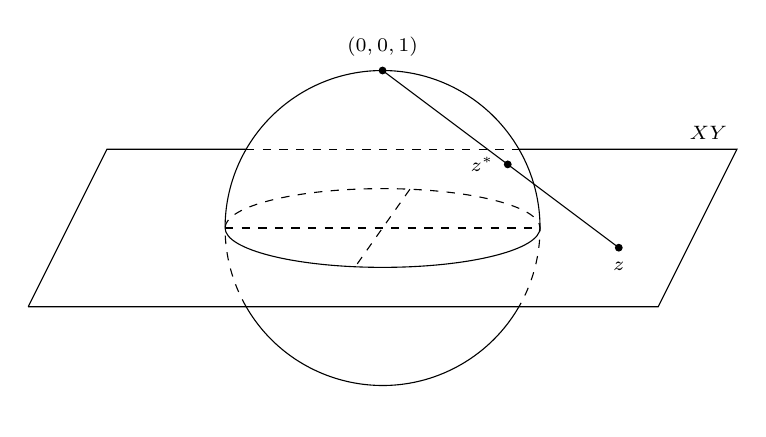
\begin{tikzpicture}
	\coordinate (A) at (3,-0.25);
	\coordinate (P) at (0,2);

	\draw (0:2cm)   arc[radius=2cm,start angle=0,end angle=180]
		  (210:2cm) arc[radius=2cm,start angle=210,end angle=330];
	\draw (180:2cm) arc[x radius=2cm, y radius=0.5cm, start angle=180,end angle=360];

	\draw [dashed] (210:2cm) 
		  arc[start angle=210,delta angle=-30,radius=2cm]
		  arc[start angle=180,delta angle=-180,x radius=2cm,y radius=0.5cm]
		  arc[start angle=0,delta angle=-30,radius=2cm];

	\draw [dashed] (80:2cm and 0.5cm) -- (260:2cm and 0.5cm);
	\draw [dashed] (150:2cm) coordinate(ul) -- (30:2cm) coordinate(ur);

	\draw (-4.5,-1) -- (3.5,-1) -- (4.5,1) node[anchor=south east] {\scriptsize$ XY $} -- (ur) (ul) -- (-3.5,1) -- (-4.5,-1);

	\draw (A) -- (P) coordinate[pos=0.47](B);
	\path (A) node[circle, fill, inner sep=1pt, label=below:{\scriptsize$ z $}]{};
	\path (B) node[circle, fill, inner sep=1pt, label=left:{\scriptsize$ z^* $}]{};
	\path (P) node[circle, fill, inner sep=1pt, label=above:{\scriptsize$ (0,0,1) $}]{};
	\draw [dashed] (-2,0) -- (2,0);
\end{tikzpicture}
	
\end{center}

\section{Rational maps}
\begin{definition}[\textbf{Rational maps}]
	A rational map is a function of the form, \[
		R(z)=\frac{P(z)}{Q(z)}
	,\] where \( P \) and \( Q \) are polynomials but not simultaneously zero polynomials.
	If \( Q(z)=0 \) and \( P \) is not the zero polynomial, then \( R \) is defined to be \( \infty \).
	Also, we define \( R(\infty) \) to be the limit of \( R(z) \) as \( z\to \infty \).
\end{definition}
We shall always assume \( P \) and \( Q \) are co-prime. We define the \textbf{degree} of a rational map \( R \) as, \[
	\deg(R)=\max\{\deg(P),\deg(Q)\}
.\] If \( R \) is a constant map (even \( \infty \)), we define, \( \deg(R)=0 \).

It is a crucial fact that if \( R \) is a rational function of degree \( d \), then \( R \) is a \( d \)-fold
map of \( \Cinf \) onto itself.


\section{Definition of Fatou and Julia sets in terms of equicontinuity}
\begin{definition}[\textbf{Fatou and Julia Sets}]
	Let \( R \) be a non-constant rational function. The Fatou set of \( R \) denoted by \( F(R) \) is 
	the maximal open subset of \( \Cinf \) on which \( \{\ror[n]\}\) is equicontinuous. The Julia set of \( R \),
	denoted by \( J(R) \) is the complement of \( F(R) \) in \( \Cinf \).
\end{definition}
By definition, \( F(R) \) is open and \( J(R) \) is compact.\\
They are denoted by simply \( F \) or \( J \) when the context is clear.

\section{Completely Invariant Components}
If \( f:X\to X \), then a subset \( D\subset X \) is:
\begin{itemize}
	\item \emph{forward invariant} under the map \( f \) if \( f(D)=D \).
	\item \emph{backward invariant} under the map \( f \) if \( f^{-1}(D)=D \).
	\item \emph{completely invariant} under the map \( f \) if it is both forward
		and backward invariant under \( f \) i.e. \( f(D)=D \) and \( f^{-1}(D)=D \).
\end{itemize}
Note that if \( f \) is surjective, i.e. \( f(X)=X \), then backward invariance implies complete invariance.
This is because, \( f(f^{-1}(D))=D \) if \( f \) is surjective. Hence, if \(f^{-1}(D)=D  \), we have \( f(D)=D \) i.e.
forward invariance.

\begin{theorem}
	If \( f:X\to X \) be a continuous, open and surjective map of a topological space \( X \) onto itself.
	If \( D\subset X \) is completely invariant under \( f \), then so are the complement \( X\bs D \), the interior \( D^0 \), 
	the boundary \( \partial D \) and the closure \( \overline{D}  \).
\end{theorem}
\begin{proof}
	Firstly, note that it is enough to prove backward invariance since \( f \) is surjective.\\
	It is trivial to see that \( X\bs D \) is completely invariant. 

	Now, since \( f \) is a continuous map,
	\( f^{-1}(D^0) \) is an open subset of \( f^{-1}(D)=D \). Hence, \( f^{-1}(D^0) \subset D^0 \). Now, since \( f \) is an open map,
	\( f(D^0) \) is an open subset of \( f(D)=D \). Hence, \( f(D^0) \subset D^0 \implies D^0 \subset f^{-1}(f(D^0)) \subset f^{-1}(D^0) \).
	Hence, \( f^{-1}(D^0)=D^0 \) and hence, \( D^0 \) is completely invariant.
	
	From the general fact for continuous maps, \( \overline{ f^{-1}(A)}\subset f^{-1}(\overline{A})  \). Hence, \( \overline{D}\subset f^{-1}(\overline{D})   \). Now, let \( x\in f^{-1}(\overline{D})  \) (or \( f(x)\in \overline{D}  \)). If \( x\not\in \overline{D}  \), then there exists and open set around \( x \), say \( U \) such that \( U\cap D=\phi \). Since \( f \) is an open map, \( f(U) \) is an open set containing \( f(x) \). Since, \( f(x)\in \overline{D}  \), \( f(U)\cap D\neq \phi \). But since, \( f^{-1}(D)=D \), \( f^{-1}(f(U)\cap D)\subset D \). But, \( f^{-1}(f(U)\cap D)\cap U\neq \phi \implies D\cap U\neq \phi\), which is a contradiction. Hence, \( \overline{D}=f^{-1}(\overline{D})   \). Hence, \( \overline{D}  \) is also completely invariant.

	Consequently, \( \partial D=\overline{D}\bs D^0  \) is also completely invariant.
\end{proof}

\begin{theorem}
	For any rational function \( R \), the Fatou and Julia sets of \( R \) i.e. \( F(R) \) and
	\( J(R) \) are completely invariant.
\end{theorem}
\begin{proof}
	First note that it is enough to prove only backward invariance because \( R \) is surjective.
	Also, we will only prove the complete invariance of \( F(R) \), the complete invariance of \( J(R) \) then follows
	from above theorem. We will use \( F \) to denote \( F(R) \).

	Let \( z_0\in R^{-1}(F) \) and let \( w_0=R(z_0)\in F \). By equicontinuity, for any \( \epsilon>0 \), \( \exists \delta>0 \) such
	that if \( \sigma(z,z_0)<\delta \), then for all \( n \in \mathbb{N} \), \( \sigma(\ror[n](w),\ror[n](w_0))<\epsilon \). By continuity of \( R \),
	there exists \( \delta'>w_0 \) such that if \( \sigma(z,w_0)<\delta' \), then \( \sigma(R(z),w_0)<\delta \) and hence,
	\( \sigma(\ror[n+1](z),\ror[n+1](z_0))<\epsilon \) for all \( n\in \mathbb{N} \). Hence, \( \{\ror[n+1]:n \in \mathbb{N}\} \) is equicontinuous 
	at \( z_0 \) and hence, so is \( \{\ror[n]:n \in \mathbb{N}\} \). Therefore, \( z_0 \in F \) and \( R^{-1}(F) \subset F \). 

	Now, let \( z_0 \in F \). To prove that \( z_0\in R^{-1}(F) \), we need to prove that \( R(z_0)\in F \). Let \( w_0=R(z_0) \).
	We have by equicontinuity, that for any \(\epsilon>0  \), \( \exists \delta>0 \) such that for all \( n \in  \mathbb{N} \), if \( \sigma(z,z_0)<\delta \), then \( \sigma(\ror[n+1](z),\ror[n+1](z_0))<\epsilon \). Now, \( N=\{z:\sigma(z,z_0)<\delta\} \) is an open set containing \( z_0 \)
	and hence, \( R(N) \) is an open set containing \( w_0 \). Now, if \( w\in R(N) \) then \( w=R(z) \) for some \( z\in N \). Hence, \[
		\sigma(\ror[n](w),\ror[n](w_0))=\sigma(\ror[n+1](z),\ror[n+1](z_0))<\epsilon
	.\] Hence, \( z_0\in R^{-1}(F) \) and \( F \subset R^{-1}(F) \).

Therefore, \( R^{-1}(F)=F \) and \( F(R) \) is completely invariant.
\end{proof} 

\begin{lemma}\label{thm1.3}
For any rational map \( R \) and a domain \( U \subset  \Cinf\), \( \partial R(U) \subset R(\partial U) \).
\end{lemma}
\begin{proof}
	Let \( w_0\in \partial R(U) \) such that it is approximated by \( R(z_n) \) for \( (z_n)_{n=1}^\infty \subset U \).
	Now, assume \( z_n\to z_0 \) (after taking a subsequence). Now, \( z_0 \) cannot lie in \( U \), otherwise \( R(z_0)=w_0 \in R(U) \).
	Since, \( R \) is an open map, \( R(U) \) is an open set and is disjoint from \( \partial R(U) \). Hence, \( z_0\in \partial U \)
	and \( R(z_0)=w_0 \in R(\partial U) \). Therefore, \( \partial R(U) \subset R(\partial U) \).
\end{proof}

\begin{lemma}\label{lem1.1}
	For a rational map \( R \), if \( F_1 \) and \( F_2 \) are two Fatou components and \( R \)
	maps a point of \( F_1 \) to a point of \( F_2 \), then \( R(F_1)=F_2 \).
\end{lemma}
\begin{proof}
Clearly, \( R(F_1)\subset F_2 \) because of forward invariance of \( F \) under \( R \) and since \( F_1 \) and \( F_2 \)
are connected components of \( F \). If \( R(F_1)\neq F_2 \), then \( \exists z \in \partial F_1 \) such that \( R(z)\in F_2 \) and
this is not possible as \( z\in \partial F_1\implies z\in J \) and \( J \) is completely invariant. Hence, \( R(F_1)=F_2 \).
\end{proof}

\begin{theorem}\label{thm1.4}
	The unbounded Fatou component of a polynomial \( P \), i.e. the Fatou component containing \( \infty \)
	is a completely invariant Fatou component. It is denoted by \( F_\infty(P) \) or simply \( F_\infty \) when
	the context is clear.
\end{theorem}
\begin{proof}
	First note that since \( P(\infty)=\infty \), we have \( P(F_\infty)=F_\infty \) by the above lemma. Hence, \( F_\infty \subset P^{-1}(F_\infty) \).
	Now assume, some point \( z_0\in P^{-1}(F_\infty) \) but \( z_0\not\in F_\infty \). By backward invariance of \( F \),  \( z_0\in F' \),
	where \( F' \) is some other Fatou component. Again, \( P(F')=F_\infty \) by above lemma. But for polynomials, we have \( P^{-1}(\infty)=\{\infty\}\). Hence, \( \infty \in F' \) and \( F' \) must be \( F_\infty \) itself. Therefore, \( P^{-1}(F_\infty)=F_\infty \) and \( F_\infty \) is completely invariant under \( P \).
\end{proof}

\begin{theorem}
	Let \( R \) be rational map and let \( E \) be a finite set which is completely invariant under \( R \). 
	Then \( E \) has atmost two elements.
\end{theorem}
\begin{proof}
	Suppose \( E \) has \( k \) elements. Now, \( R \) acts as a permutation of \( E \) and hence for some integer \( s \),
	\( \ror[s] \) acts as an identity map on \( E \). Now, suppose \( \ror[s] \) has degree \( d \). It follows that for any \( z_0\in E \),
	\( \ror[s](z)=z_0 \) has solution \( z_0 \) with multiplicity \( d \). Applying the Riemann-Hurwitz formula, (in the next section) \[
		k(d-1)\le 2d-2
	\] and hence, \( k\le 2 \).
\end{proof}


\section{Valency and the Riemann-Hurwitz formula}
Let \( f \) be a holomorphic map on the complex plane. Then, near a point \( z_0 \), \( f \) has the Taylor expansion,\[
	f(z)=f(z_0)+a_k(z-z_0)^k+\ldots 
,\]  where \( a_k\neq 0 \) and \( k\ge 1 \). Then, we define the valency of \( f \) at \( z_0 \),
\( v_f(z_0)=k \).

For \( f:X\to Y \) where \( X \) and \( Y \) are Riemann surfaces, we have local analytic co-ordinates near \( z_0 \)
and \( f(z_0) \) such that \( f \) has the form \( f(z)=a_kz^k+\ldots  \), (\( a_k\neq 0 \) and \( k\ge 1 \))
then again we define the valency of \( f \)
at \( z_0 \) as \( v_f(z_0)=k \). The valency is independent of the choice of co-ordinates.

\begin{definition}[Deficiency]
	We define the deficiency of \( f \) over a set \( A \) as, \[
		\delta_f(A)=\sum_{z\in A} (v_f(z)-1)
	.\] 
\end{definition}

\begin{theorem}[\textbf{Generalized Riemann-Hurwitz formula}]
	Let \( X \) and \( Y \) be Riemann surfaces and \( f:X\to Y \) be a complex analytic map of degree \( d \). Then,
	\[
		\chi(X)+\delta_f(X)=d\chi(Y)
	,\] where \( \chi(X) \) denotes the Euler characteristic of \( X \).\\
	For a compact, connected and orientable surface \( S \), the Euler characteristic \( \chi(S)=2-2g \),
	where \( g \) is the genus of \( S \). Hence, if \( X \) and \( Y \) are compact Riemann surfaces,
	we get the following formula (after multiplying both sides by \( -1 \)),\[
		2g(X)-2=d(2g(Y)-2)+\delta_f(X)
	.\] 
\end{theorem}

\begin{theorem}[\textbf{Riemann-Hurwitz Formula} (version 1)]
Now, genus of a sphere is zero and hence, \( g(\Cinf)=0 \).
For a rational map, which is a \( d \)-fold map of the complex sphere onto itself, we have,
\begin{align*}
	\implies & 2g(\Cinf)-2=d(2g(\Cinf)-2)+\delta_R(\Cinf)\\
	\implies &\delta_R(\Cinf)=2d-2\\
	\implies &\sum_{z\in \Cinf}(v_R(z)-1)=2d-2
.\end{align*}
\end{theorem}

\begin{theorem}[\textbf{Riemann-Hurwitz Formula}  (version 2)]
	Let \( F_0 \) and \( F_1 \) be components of the Fatou set \( F \) of a rational map \( R \)
	and \( R \) maps \( F_0 \) into \( F_1 \). Then, for some integer \( m \), \( R \) is an \( m \)-fold
	map of \( F_0 \) onto \( F_1 \) and \[
		\chi(F_0)+\delta_R(F_0)=m\chi(F_1)
	.\] 
\end{theorem}

\section{Equicontinuity and Normality}
There is another criterion that we use more in practice to define Fatou sets.
\begin{definition}[\textbf{Normal Families}]
	A family of maps, \( \mathcal{F} \) of maps from metric space \( (X_1,d_1) \) to \( (X_2,d_2) \) is said to be a normal family in \( X_1 \),
	if every infinite sequence of function in \( \mathcal{F} \) has a subsequence which converges locally uniformly on \( X_1 \).
\end{definition}

The Arzela-Ascoli theorem connects equicontinuity and normality. This is one of the many forms of the theorem, which is suitable for our use.
\begin{AAT}
	Let \( D \) be a domain on the complex sphere and let \( \mathcal{F} \) be a family of continuous maps defined on \( D \).
	Then, \( \mathcal{F} \) is equicontinuous in \( D \) if and only if  it is a normal family in \( D \).
\end{AAT}
Thus, we can redefine the Fatou set of \( R \) as the maximal open set of \( \Cinf \) 
on which the family \( \{\ror[n]\} \) is normal.

\begin{theorem}[\textbf{Vitali's Theorem}]
		Let \( D \) be a subdomain of complex sphere. Suppose \( \{f_n\}_{n\in\mathbb{N}} \)	be a family of analytic maps normal in \( D \). Also suppose, \( \{f_n\} \) converges pointwise on some subset \( W\subset D \) such that \( W \) contains a limit point in \( D \). Then, \( f(z):=\lim_{n \to \infty} f_n(z), z\in W \) extends to an analytic function \( F \) on \( D \) and \( f_n\to F \) locally uniformly in \( D \).
\end{theorem}
\begin{proof}
	As \( \{f_n\} \) is a normal family, there is a subsequence of \( (f_n) \) which converges locally uniformly in \( D \)
	to some analytic function \( F \) and \( F=f \) on \( W \).

	Now, assume \( (f_n) \) fails to converge locally uniformly to \( F \) on \( D \). Then, there is some subsequence \( (g_n) \)
	of \( (f_n) \) and \( \epsilon>0 \) such that for all \( n \) and all \( z\in K \),\[
		\sigma(g_n(z),F(z))\ge \epsilon
	.\] But again by normality, there is a subsequence \( (h_n) \) of \( (g_n) \) which converges locally uniformly in \( D \)
	to some analytic function \( h \). Clearly, \( h=F=f \) on \( W \) and since \( W \) has a limit point in \( D \),
	\( h=F \) throughout \( D \) by the Identity theorem. It follows that, \[
		\sigma(h_n(z),F(z))\to 0
	\]  uniformly in \( K \). This is a contradiction as \( (h_n) \) is a subsequence of \( (g_n) \).
	Hence, \( (f_n) \) converges locally uniformly to \( F=f \) on \( D \).
\end{proof}

\begin{corollary}\label{lem1.2}
	If \( \alpha \) is a (super)-attracting fixed point of a rational map \( R \) and \( F_\alpha \) is the
	Fatou component containing \( \alpha \) then \( \ror[n](z)\to \alpha \)
	locally uniformly in \( F_\alpha \).
\end{corollary}

We now state one of the most important theorem for normal families, the \emph{Montel's Fundamental Normality Criterion}.
It provides us with a very easy way to check if some family of maps is normal on a domain of the complex sphere.
\begin{theorem}[\textbf{Montel's Fundamental Normality Criterion}]
	Let \( \mathcal{F} \) be a family of maps, each analytic in a domain \( D \) of the complex sphere.
	Suppose \( \exists m>0 \) and for each \( f\in \mathcal{F} \), three distinct points \( a_f,b_f \) and \( c_f \) such that,
	\begin{enumerate}
		\item \( f(D) \) does not contain \( a_f,b_f \) and \( c_f \),
		\item \(\min\{\sigma(a_f,b_f),\sigma(b_f,c_f),\sigma(c_f,a_f)\}\geq m\),
	\end{enumerate}
	then \( \mathcal{F} \) is normal in \( D \).
\end{theorem}

\section{Exceptional points and minimality of the Julia set}
\begin{theorem}[\textbf{Minimality of \( J \)}]
	Let \( R \) be a rational map with \( \deg(R)\ge 2 \) and suppose that \( E \) is a closed, completely invariant
	subset of the complex sphere. Then either,
	\begin{enumerate}
		\item \( E \) has atmost two elements and \( E \subset E(R) \subset F(R) \).
		\item \( E \) is infinite and \( J(R) \subset E \).
	\end{enumerate}
\end{theorem}
\begin{proof}
	We know that either \( E \) has atmost two points or it is infinte. If \( E \) is finite, then \( E \) contains
	only exceptional points which lie in \( F(R) \). Now, suppose \( E \) is infinite. As \( E \) is completely invariant, so
	is its complement, say \( G \). Hence, \( \ror[n] \) maps \( G \) into itself for each \( n \in \mathbb{N} \). Hence, applying 
	Montel's Fundamental Normality Criterion, while choosing \( a_f,b_f \) and \( c_f \) to be any three points in \( E \),
we see that \( \{\ror[n]\} \) is a normal family in \( G \). Hence, \( G \subset F \implies J \subset G^c=E \).
\end{proof}
\noindent This result can also be stated as:\\
\textbf{\( J \) is the smallest, closed completely invariant set with atleast three points.}

\begin{corollary}\label{thm1.2}
	If \( R \) is a rational function, with \( \deg(R)\ge 2 \), and \( F_0 \) is
	a completely invariant Fatou component of \( R \), then, \( \partial F_0=J \).
\end{corollary}
\begin{proof}
	As \( F_0 \) is completely invariant, so is \( \overline{F_0}  \). By minimality of \( J \), \( J\subset \overline{F_0}  \).
	As \( J \) is disjoint from \( F_0 \), \( J=\partial F_0 \).
\end{proof}

\section{Connectivity}
\begin{definition}[Connectivity]
	The connectivity of a domain \( D \subset \Cinf \) is defined as the number
	of components of \( \partial D \).
\end{definition}

\begin{theorem}\label{thm1.1}
	The following are equivalent for a domain \( D\subset \Cinf \):
	\begin{enumerate}
		\item \( D \) is simply connected.
		\item \( D^c \) is connected.
		\item \( \partial D \) is connected or \( c(D)=1 \).
	\end{enumerate}
\end{theorem}
\begin{proof}
	\( D^c \) being connected can be taken as the definition of \( D \) being simply connected, as it is done by Ahlfors \parencite{ahlfors}.
	Later it is this definition of simply connected, which is used to prove the Riemann mapping theorem, which proves biholomorphism
	between simply connected sets and the unit disc which is actually simply connected.

	We will prove the equivalence of \emph{1} and \emph{3}.

	If \( D \) is not simply connected, then there is a simple closed curve \( \gamma \) in \( D \) which 
	separtes the complement of \( D \), proving that \( \partial D \) is disconnected.

	Now, suppose that \( \partial D \) is disconnected. Then there is a simple closed curve \( \gamma \) which
	separtes \( \partial D \) into two disjoint subsets \( A \) and \( B \). Since, \( D \) is path-connected and
	\( D \) is arbitrarily close to \( A \) and \( B \), \( D \) intersects \( \gamma \). By construction, \(\gamma\) does
	not intersect \( \partial D \) and hence, \( \gamma\) lies in \( D \). Thus, \( A \) and \( B \) lie in different
	components of the complement of \( D \) and hence, \( D \) cannot be simply connected.
\end{proof}

\noindent \textbf{Note:} If \( D \) is simply connected, we have \( c(D)=1 \) and \( \chi(D)=1 \).\\
More generally, \( \chi(D)=2-c(D) \).


